\documentclass[12pt,a4paper]{scrartcl}

%========================================================================================
%SPRACHE

\usepackage[ngerman]{babel} 
\usepackage[T1]{fontenc} 				% richtige Silbentrennung
\usepackage[utf8]{inputenc}
%========================================================================================
%DARSTELLUNG

\usepackage[small,compact]{titlesec} 		% Verkleinerung von Section-Ueberschriften
\usepackage{graphicx}				  	% Einbinden von Graphiken .ps, .pdf, .png

\usepackage{amsmath}					% mathematische Symbole
\usepackage {ulem} 						%\emph{Text}: Text wird unterstrichen
\setlength{\parindent}{0pt}				% Zeile nach Absatz einruecken 1pt oder nicht 0pt.

\usepackage{float} % alles möglichen Sachen mit [h] an die richtige Stelle zwingen
%========================================================================================
%FARBEN

\usepackage[usenames,dvipsnames]{color}	

									%Apricot 	Aquamarine 	Bittersweet 	Black
									%Blue 	BlueGreen 	BlueViolet 	BrickRed
									%Brown 	BurntOrange 	CadetBlue 	CarnationPink
									%Cerulean 	CornflowerBlue 	Cyan 	Dandelion
									%DarkOrchid 	Emerald 	ForestGreen 	Fuchsia
									%Goldenrod 	Gray 	Green 	GreenYellow
									%JungleGreen 	Lavender 	LimeGreen 	Magenta
									%Mahogany 	Maroon 	Melon 	MidnightBlue
									%Mulberry 	NavyBlue 	OliveGreen 	Orange
									%OrangeRed 	Orchid 	Peach 	Periwinkle
									%PineGreen 	Plum 	ProcessBlue 	Purple
									%RawSienna 	Red 	RedOrange 	RedViolet
									%Rhodamine 	RoyalBlue 	RoyalPurple 	RubineRed
									%Salmon 	SeaGreen 	Sepia 	SkyBlue
									%SpringGreen 	Tan 	TealBlue 	Thistle
									%Turquoise 	Violet 	VioletRed 	White
									%WildStrawberry 	Yellow 	YellowGreen 	YellowOrange
									
									% verwenden mit: 
									% \pagecolor{declared-color}
									% {\color{declared-color} text}
									% \colorbox{declared-color1}{\color{declared-color2} text}

									%========================================================================================
%Zur Einbindung von Programmiertexten mit:
				% \begin{lstlisting}
				%put your code here
				%\end{lstlisting}
				
\usepackage{listings}
\lstset{ %
language=bash,                			% the language of the code
basicstyle=\footnotesize,       			% the size of the fonts that are used for the code
numbers=left,                   				% where to put the line-numbers
numberstyle=\footnotesize,      			% the size of the fonts that are used for the line-numbers
stepnumber=2,                   				% the step between two line-numbers. If it's 1, each line 
                                					% will be numbered
numbersep=5pt,                  			% how far the line-numbers are from the code
backgroundcolor=\color{white},  		% choose the background color. You must add \usepackage{color}
showspaces=false,               			% show spaces adding particular underscores
showstringspaces=false,        		 	% underline spaces within strings
showtabs=false,                 				% show tabs within strings adding particular underscores
frame=single,                   				% adds a frame around the code
tabsize=2,                      				% sets default tabsize to 2 spaces
captionpos=b,                   				% sets the caption-position to bottom
breaklines=true,                				% sets automatic line breaking
breakatwhitespace=false,        			% sets if automatic breaks should only happen at whitespace
title=\lstname,                 				% show the filename of files included with \lstinputlisting;
                                					% also try caption instead of title
}
%========================================================================================


%LOAD FANCYHDR fuer Kopf- und Fu{ß}zeilen
\usepackage{fancyhdr}					% Paket laden	für einfache Handhabung von Kopf-und Fu{ß}zeile
\pagestyle{fancy}							
\fancyhf{}
\fancyhead[L]{\small{\textbf{Potentialtheorie \\ Semesterabschlussarbeit}}}
\fancyhead[R]{\small{Sebastian Beyer \\ 25. Februar 2013}}
\fancyfoot[C]{\thepage} 			%Seitennummer



\usepackage{subfigure}

\addto\captionsngerman{
\renewcommand{\figurename}{Abb.}
\renewcommand{\tablename}{Tab.}
}

\usepackage{booktabs}




\begin{document}


\begin{figure}[htb]
\centering
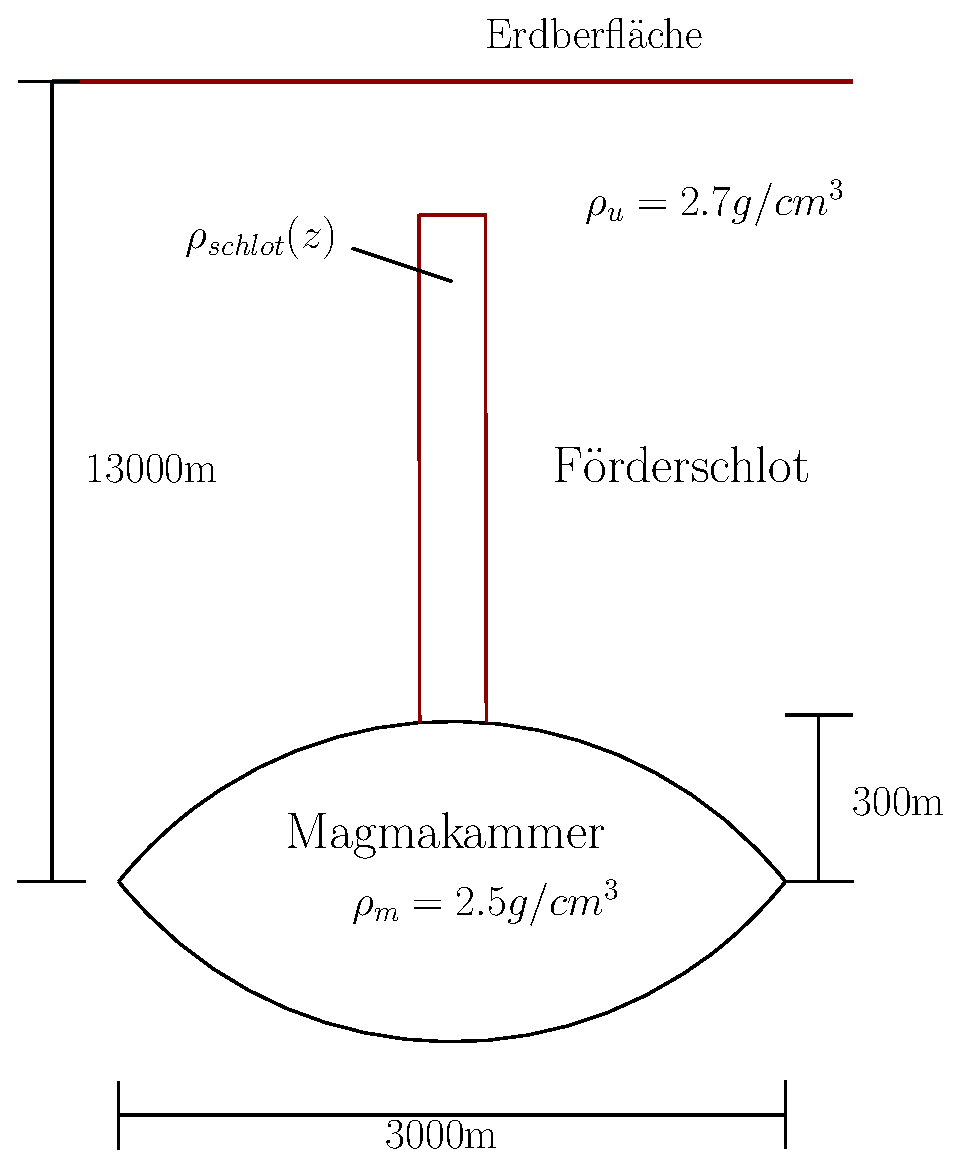
\includegraphics[width=0.4\textwidth]{../figures/geometry}
\caption{Geometrie}
\label{geometry}
\end{figure}

\begin{figure}[htb]
\centering
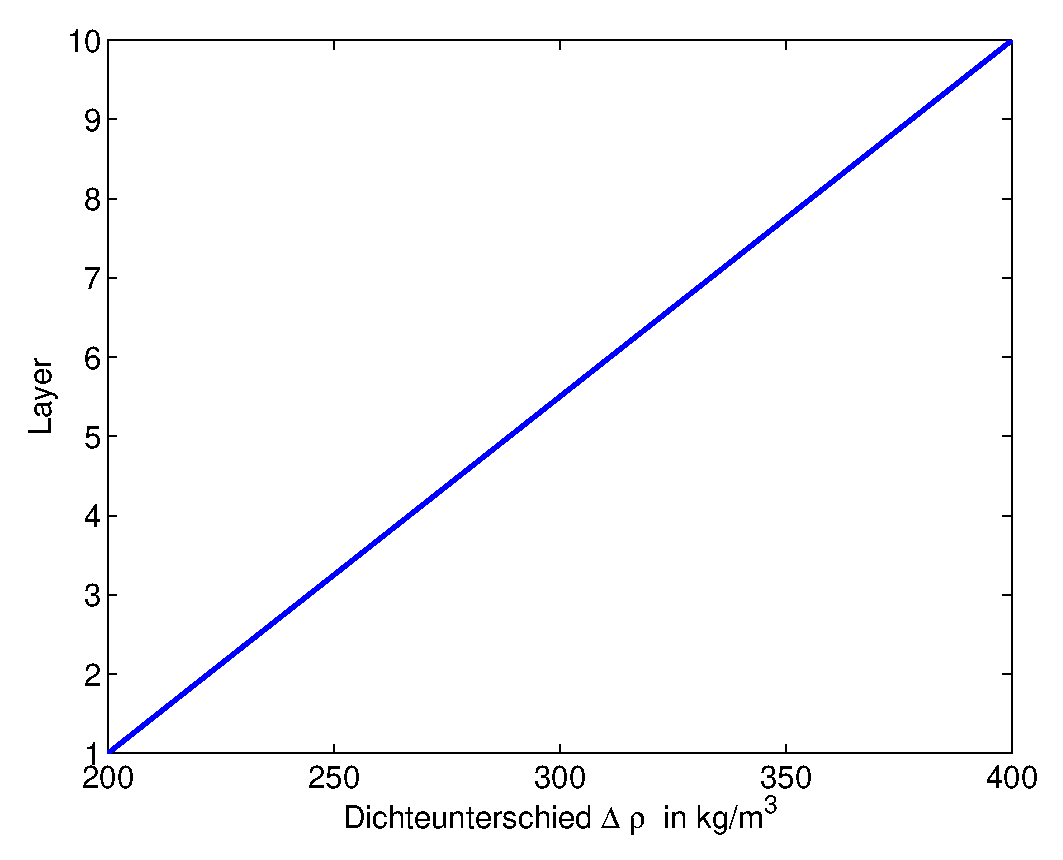
\includegraphics[width=0.6\textwidth]{../figures/rho_model}
\caption{rho model}
\label{rhomodel}
\end{figure}

\begin{figure}[htb]
\centering
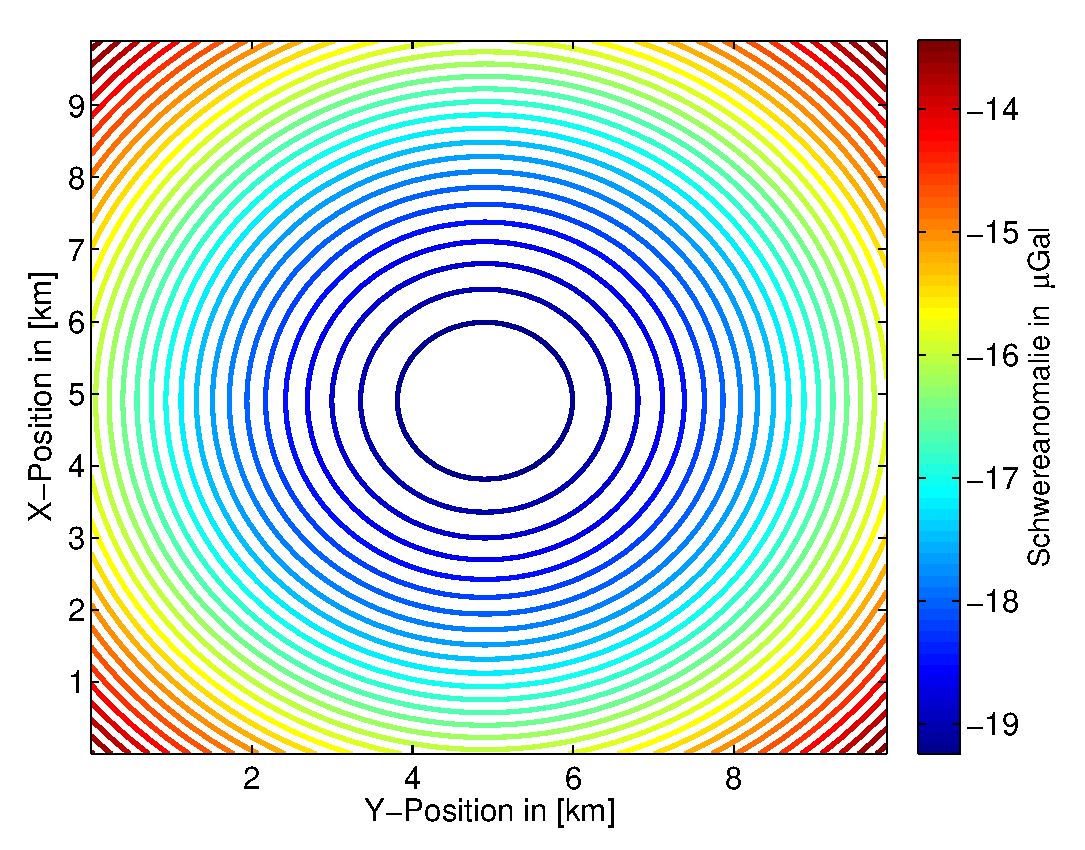
\includegraphics[width=0.8\textwidth]{../figures/2dchamber_contour}
\caption{2dchamber}
\label{2dchamber}
\end{figure}


\begin{figure}[htb]
\centering
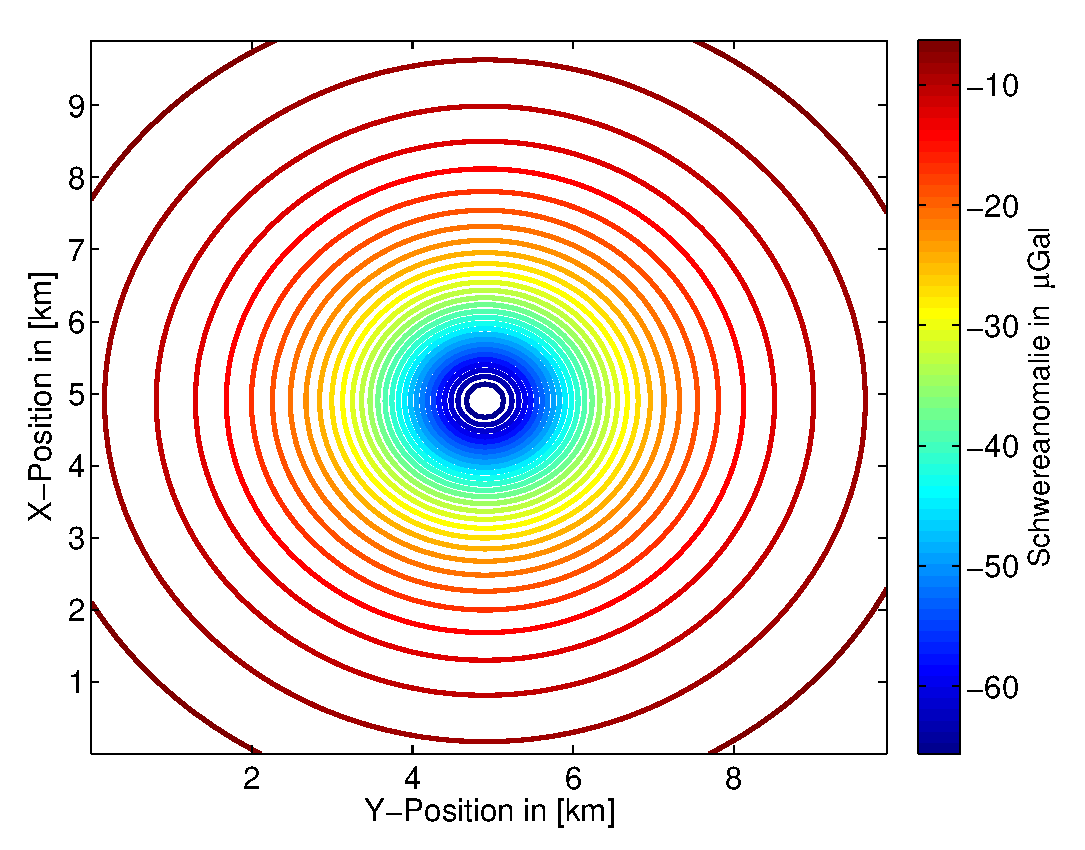
\includegraphics[width=0.8\textwidth]{../figures/2dconduit_contour}
\caption{2dconduit}
\label{2dconduit}
\end{figure}

\begin{figure}[htb]
\centering
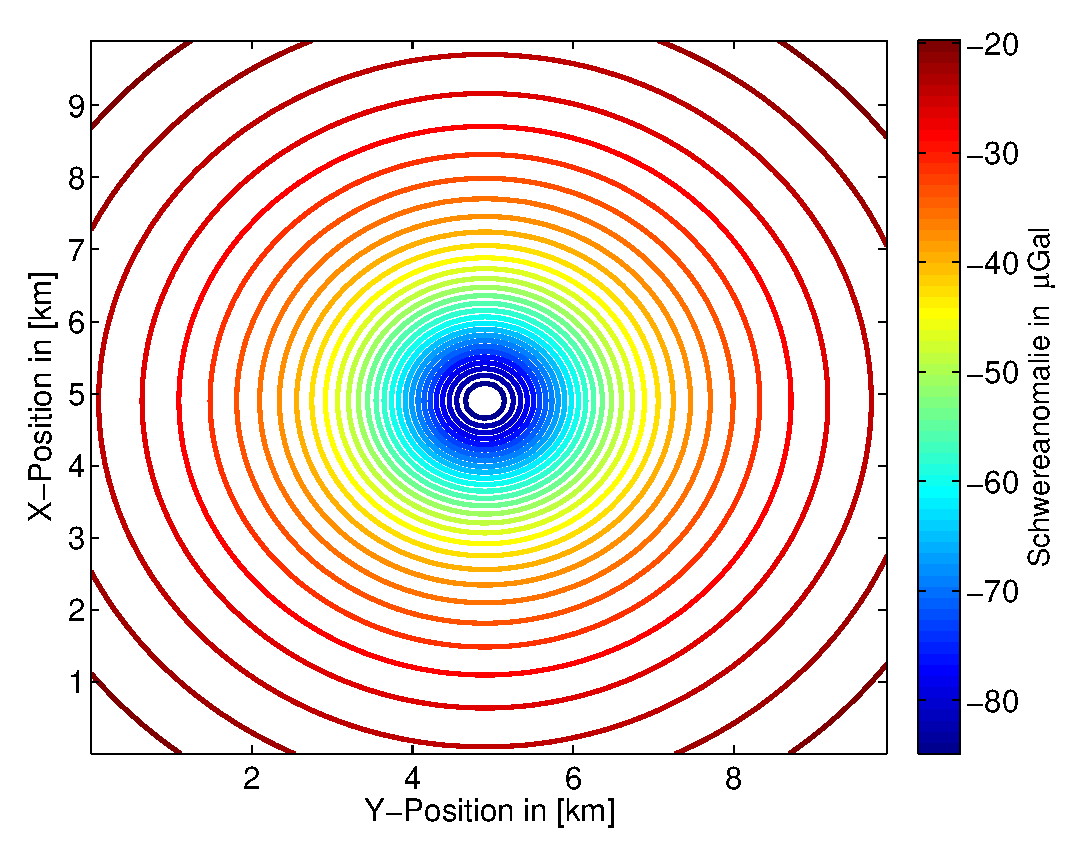
\includegraphics[width=0.8\textwidth]{../figures/2dwhole_contour}
\caption{2dwhole}
\label{2dwhole}
\end{figure}

\begin{figure}[htb]
\centering
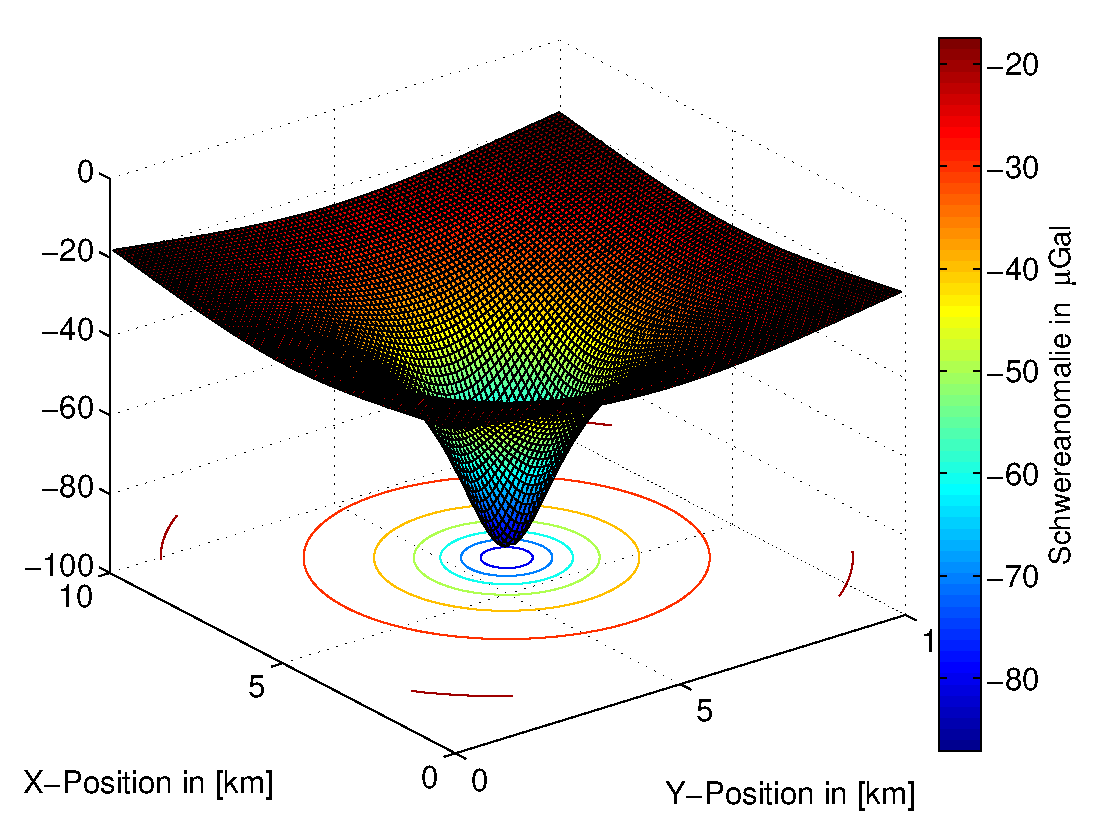
\includegraphics[width=0.8\textwidth]{../figures/2dwhole_surfc}
\caption{2dsurfc}
\label{2dsurfc}
\end{figure}


\begin{figure}[htb]
\centering
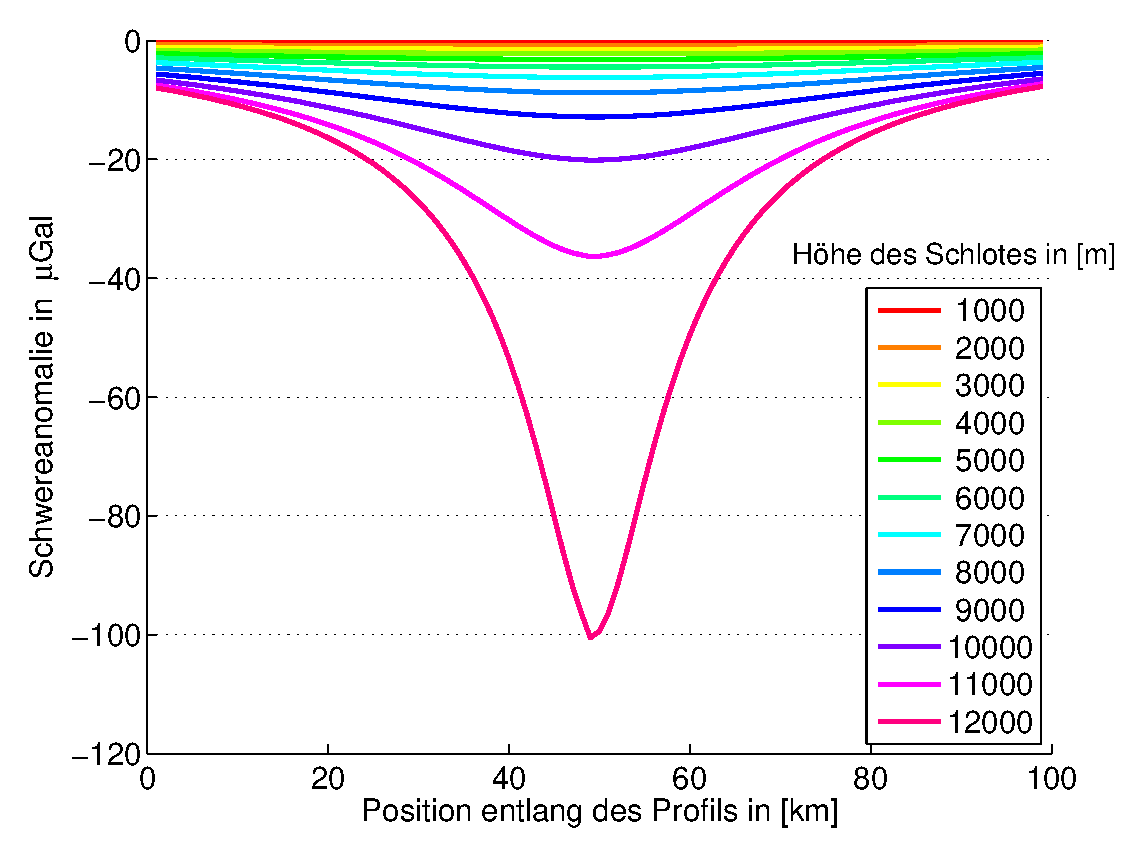
\includegraphics[width=0.8\textwidth]{../figures/var_height}
\caption{variation of height}
\label{varheight}
\end{figure}




\end{document}



